\documentclass[11pt]{article}
\usepackage[margin=2.5cm]{geometry}
\usepackage[utf8]{inputenc}
\usepackage[T1]{fontenc}
\usepackage{graphicx}
\usepackage{booktabs}
\usepackage{longtable}
\usepackage{xcolor}
\usepackage{hyperref}
\usepackage{siunitx}
\usepackage{caption}
\hypersetup{colorlinks=false, pdfborder={0 0 0}}

\renewcommand{\figurename}{Figura}
\renewcommand{\tablename}{Tabla}
\renewcommand{\contentsname}{Índice}

\definecolor{okgreen}{RGB}{0,120,60}
\definecolor{warnred}{RGB}{180,30,30}
\definecolor{sugamber}{RGB}{170,110,0}

\title{ComplexCalc-HW — Revisión del esquema de alimentación}
\author{}
\date{}

\begin{document}
\maketitle
\vspace{-1.3cm}

\section{Propósito}

Este documento resume los requisitos oficiales de alimentación del
STM32F411CEUx (datasheet DocID026289 Rev.\,7, ST\-Microelectronics) para el
paquete \textbf{UFQFPN48}, y los compara contra lo que actualmente está
routeado en \texttt{design/\allowbreak ComplexCalc/\allowbreak
ComplexCalc.kicad\_sch} del repositorio
\texttt{UAA-F14/\allowbreak ComplexCalc-HW}. Todas las figuras y tablas de referencia son
capturas directas del datasheet oficial.

\section{Pinout real: UFQFPN48}

La Figura~\ref{fig:pinout} (Figura~10 del datasheet, página~34) muestra la
asignación exacta de pines del paquete que se usa en esta placa. De ahí se
confirma:

\begin{itemize}
  \item \textbf{3 pines VDD}: 24, 36, 48
  \item \textbf{3 pines VSS}: 23, 35, 47
  \item \textbf{1 solo pin VCAP\_1} (pin 22) — este paquete \emph{no} trae
        VCAP\_2 (esa señal solo existe en LQFP100 y UFBGA100)
  \item VBAT: pin 1
  \item VDDA/VREF+: pin 9 · VSSA/VREF-: pin 8
  \item NRST: pin 7 · BOOT0: pin 44
\end{itemize}

\begin{figure}[h]
  \centering
  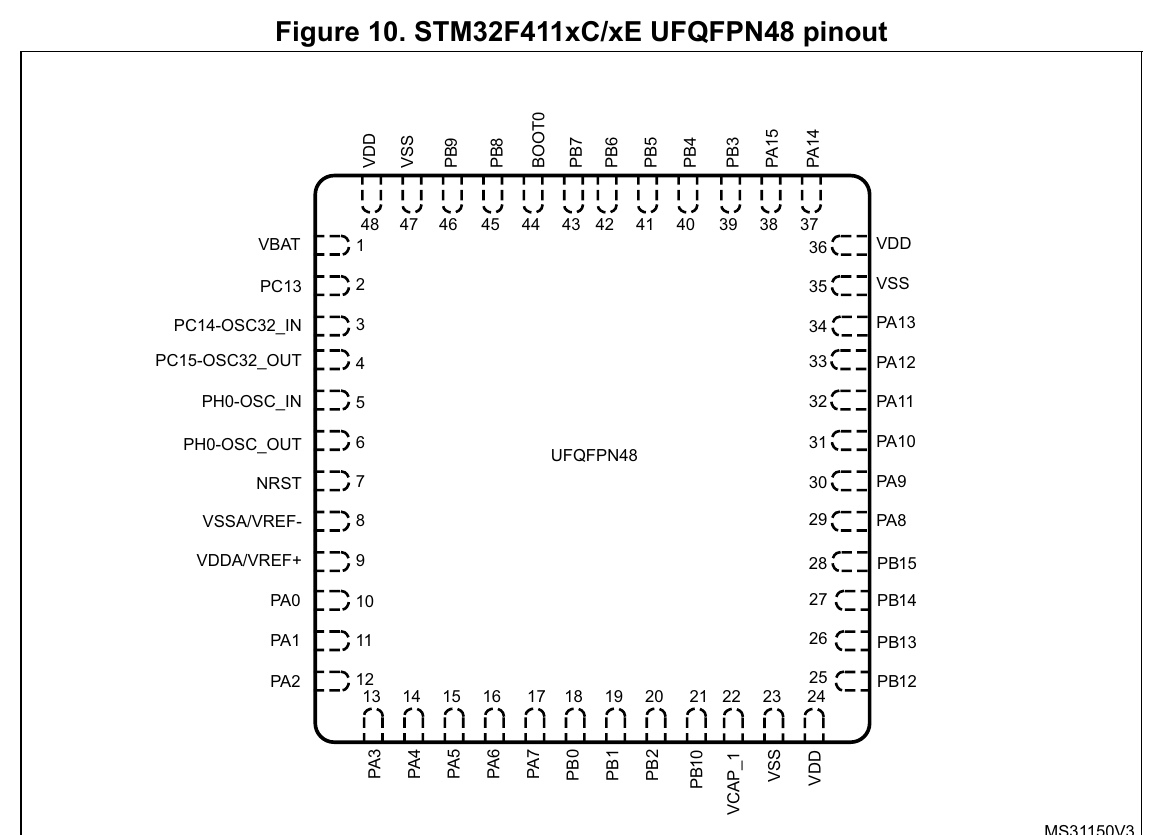
\includegraphics[width=0.58\textwidth]{figs/pinout-034-crop.png}
  \caption{Pinout UFQFPN48 — Figura 10, datasheet STM32F411xC/xE, pág.~34}
  \label{fig:pinout}
\end{figure}

\clearpage
\section{Esquema oficial de alimentación}

La Figura~\ref{fig:powerscheme} (Figura~17, Sección 6.1.6, página~59) es el
esquema de referencia de ST para el desacoplo de cada rama de alimentación.

\begin{figure}[h]
  \centering
  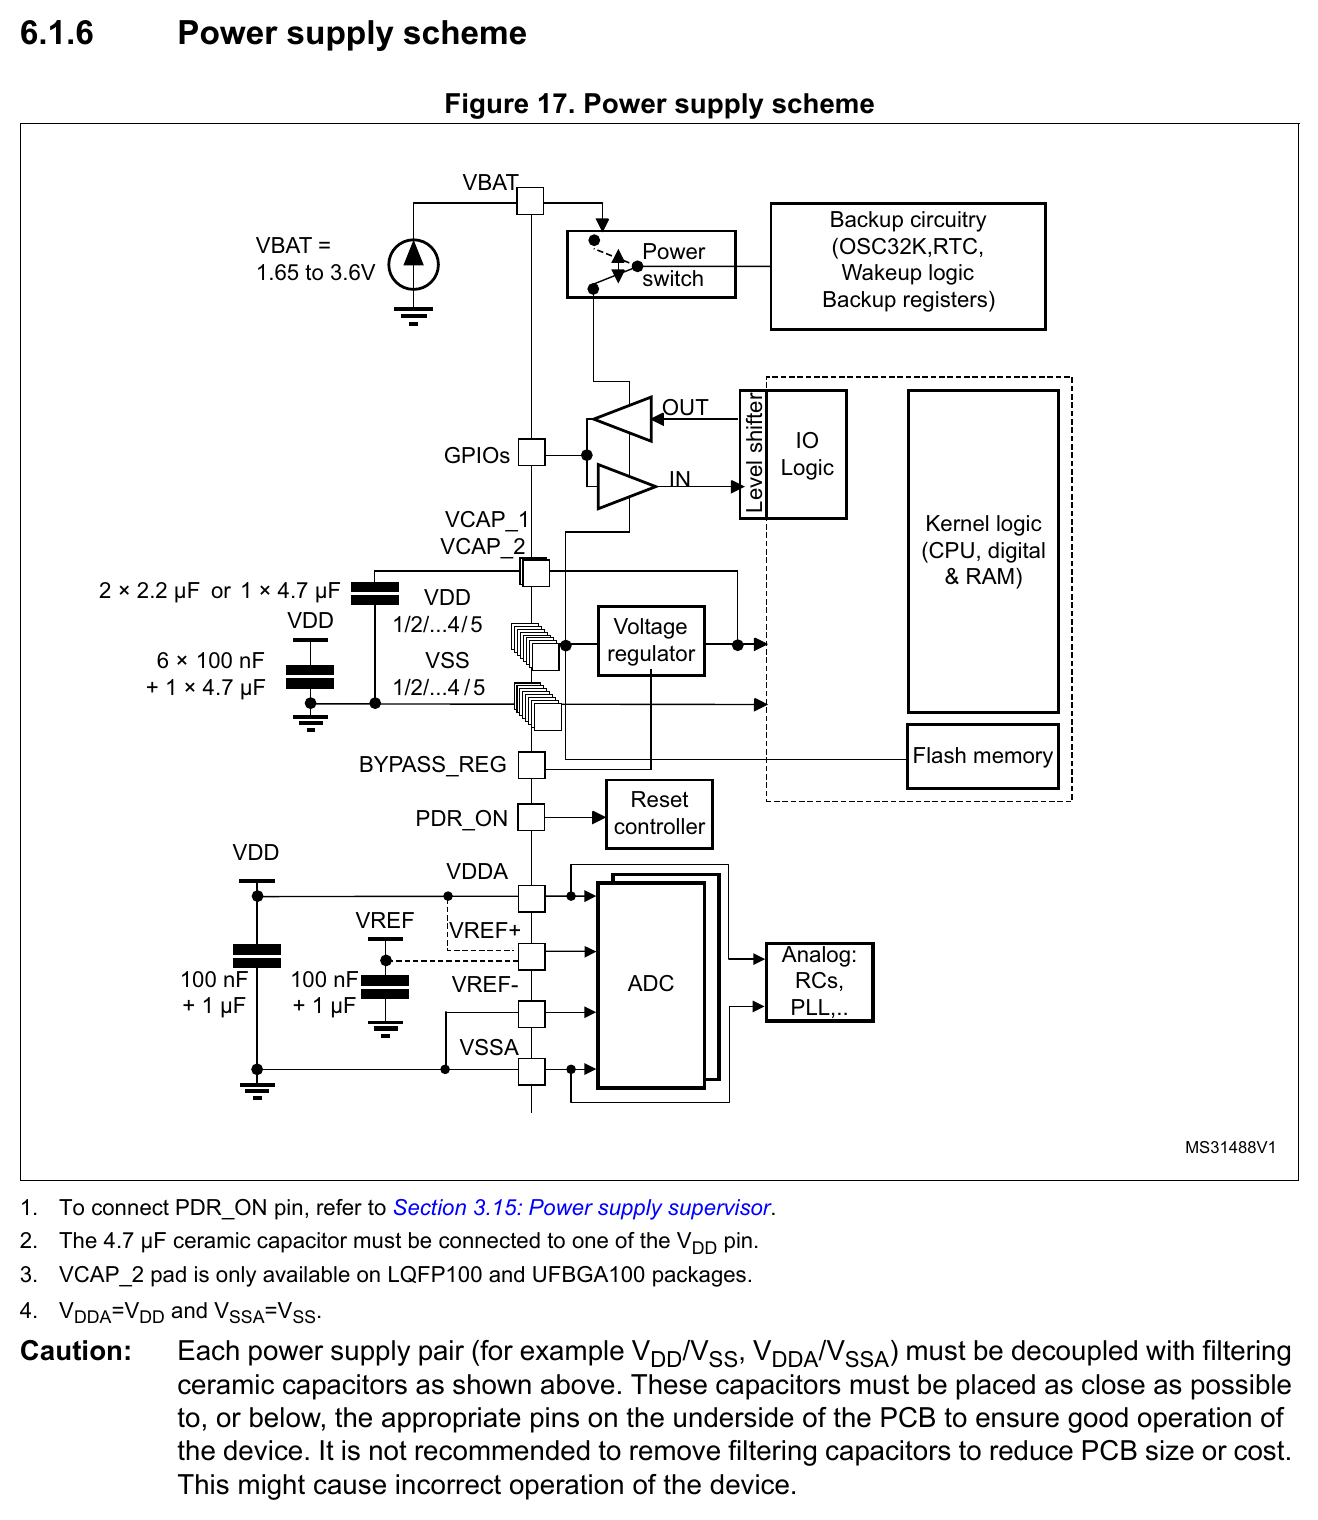
\includegraphics[width=0.72\textwidth,height=0.78\textheight,keepaspectratio]{figs/powerscheme-059-crop.png}
  \caption{Power supply scheme — Figura 17, Sección 6.1.6, pág.~59}
  \label{fig:powerscheme}
\end{figure}

\newpage
\section{Capacitor de VCAP para paquetes de un solo pin}

La Tabla~\ref{fig:vcaptable} (Tabla~16, Sección 6.3.2, página~65) da el valor
exacto que aplica específicamente cuando el paquete solo trae un pin VCAP
(nuestro caso).

\begin{figure}[h]
  \centering
  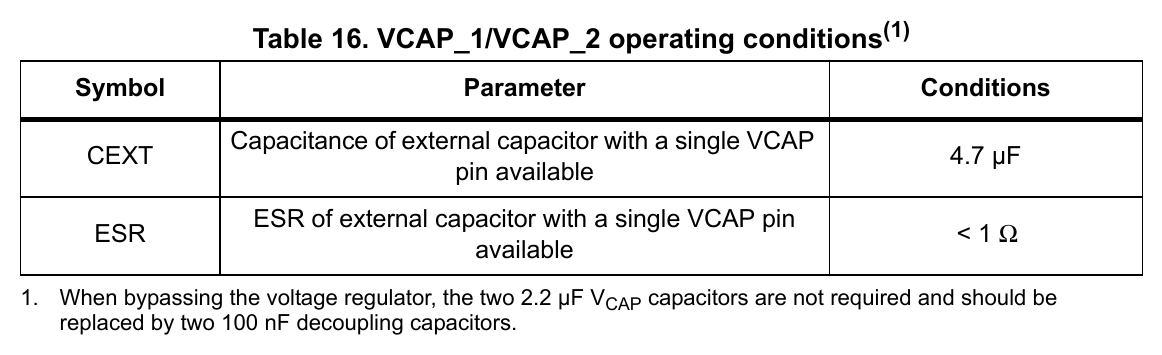
\includegraphics[width=0.8\textwidth]{figs/vcaptable-065-crop.png}
  \caption{VCAP\_1/VCAP\_2 operating conditions — Tabla 16, Sección 6.3.2, pág.~65}
  \label{fig:vcaptable}
\end{figure}

\section{Resumen: valores requeridos por pin}

\begin{longtable}{p{3.2cm}p{4.5cm}p{6cm}}
\toprule
\textbf{Pin(es)} & \textbf{Capacitor(es) requerido(s)} & \textbf{Fuente} \\
\midrule
\endhead
VDD / VSS (pines 24/23, 36/35, 48/47) &
  100\,nF por cada par VDD/VSS (3 en total) + 1$\times$4.7\,µF en cualquiera
  de los VDD &
  Figura~17, nota~2 \\
VCAP\_1 (pin 22) $\rightarrow$ GND &
  \textbf{4.7\,µF cerámico, ESR $<$ 1\,$\Omega$} (paquete de un solo VCAP) &
  Tabla~16, Sección~6.3.2 \\
VDDA/VREF+ (pin 9) $\leftrightarrow$ VSSA/VREF- (pin 8) &
  100\,nF + 1\,µF (un solo par: en este paquete VDDA y VREF+ comparten pin) &
  Figura~17 \\
VBAT (pin 1) &
  100\,nF, o conexión directa a VDD si no se usa batería de respaldo &
  Figura~17 \\
NRST (pin 7) &
  Ya trae pull-up interno — capacitor externo (100\,nF, opcional) solo
  mejora inmunidad a EMI, no es obligatorio &
  Tabla~7 (leyenda NRST) \\
BOOT0 (pin 44) &
  Sin bias interno — resistencia externa (típico 10\,k$\Omega$ pull-down
  para bootear de flash) &
  Sección 3.13 ``Boot modes'' \\
\bottomrule
\end{longtable}

\clearpage
\section{Comparación contra lo routeado en el esquemático real}

Extraído del netlist de \texttt{ComplexCalc.kicad\_sch} (exportado con
\texttt{kicad-cli}) el 2 de septiembre de 2026.

\begin{longtable}{p{3.5cm}p{3.2cm}p{3.2cm}p{4cm}}
\toprule
\textbf{Punto revisado} & \textbf{Requerido} & \textbf{En el esquemático} & \textbf{Veredicto} \\
\midrule
\endhead
VCAP\_1 (C14) & 4.7\,µF, ESR$<$1$\Omega$ & \textbf{2.2\,µF} &
  \textcolor{warnred}{\textbf{Por debajo del valor requerido}} — 2.2\,µF es el
  valor para paquetes con \emph{dos} pines VCAP, no uno solo. \\
VBAT (pin 1) & Atado a batería o a VDD & \textbf{Sin conexión (net aislada)} &
  \textcolor{warnred}{\textbf{Flotando}} — no está ni en el net de 3.3V ni tiene
  capacitor. \\
VDD/VSS (3 pares) & 3$\times$100\,nF + 1 bulk & C10, C11, C12 (100\,nF c/u)
  + C13 (1\,µF) + C8 (22\,µF) & \textcolor{okgreen}{Cumple} — bulk incluso más
  grande de lo mínimo pedido. \\
VDDA/VREF+ (pin 9) & 100\,nF + 1\,µF local & Mismo net de 3.3\,V que VDD,
  con C13 (1\,µF) presente & \textcolor{okgreen}{Cumple eléctricamente} — no se
  pudo verificar cercanía física del capacitor al pin desde el esquemático
  (revisar en el layout). \\
NRST & Pull-up interno ya suficiente; cap.\ típico 100\,nF & R4 (10\,k$\Omega$
  externo, redundante) + C9 (\textbf{1\,µF}, no 100\,nF) &
  \textcolor{sugamber}{\textbf{Sugerido bajar a 100\,nF}} — no es un error
  (sigue siendo funcional), pero 1\,µF alarga el tiempo de reset más de lo
  necesario. Confirmado contra el esquemático real del BlackPill (WeAct
  Studio): su circuito de reset usa exactamente \textbf{100\,nF} en el mismo
  nodo. \\
BOOT0 (R5) & Pull-down $\sim$10\,k$\Omega$ & 10\,k$\Omega$ &
  \textcolor{okgreen}{Correcto} \\
BOOT1/PB2 (R6) & Definir nivel & 10\,k$\Omega$ pull &
  \textcolor{okgreen}{Correcto} \\
Cristal HSE (Y1) & Coincidir con \texttt{RCC.HSE\_VALUE} en firmware &
  Y1 = \textbf{8\,MHz} físico, pero el \texttt{.ioc} tiene
  \texttt{HSE\_VALUE=25000000} & \textcolor{warnred}{\textbf{Revisar}} — si el
  firmware llega a habilitar HSE, el árbol de reloj debe recalcularse para
  8\,MHz, no 25\,MHz. \\
Regulador (U2) & --- & \textbf{AMS1117-3.3} (no NCP1117-3.3) &
  Nota de documentación: corregido en el README del repo. \\
\bottomrule
\end{longtable}

\section{Acciones recomendadas}

\begin{enumerate}
  \item Cambiar C14 de 2.2\,µF a \textbf{4.7\,µF} en VCAP\_1.
  \item Conectar VBAT (pin 1) a la red de 3.3\,V (o dejar un footprint de
        100\,nF si en el futuro se agrega batería de respaldo real para el
        RTC).
  \item Bajar C9 (NRST) de 1\,µF a \textbf{100\,nF} — valor de libro y el que
        usa el BlackPill real de referencia en el mismo nodo.
  \item Antes de habilitar el HSE en firmware, corregir
        \texttt{RCC.HSE\_VALUE} a 8\,MHz en el \texttt{.ioc} y regenerar el
        árbol de reloj en STM32CubeMX.
  \item Verificar en el layout físico (no solo el esquemático) que los
        capacitores de VDD/VDDA queden lo más cerca posible de sus pines
        respectivos, dado que la capa inferior ya está ocupada por el
        teclado matricial.
\end{enumerate}

\end{document}
